%!TeX  root  =  user_guide.tex

\chapter{Использование модулей ядра QGIS}\label{sec:core_plugins}\index{модули!ядра}

% когда переработка раздела будет завершена,
% раскоментируйте следующую строку:
% \updatedisclaimer

{\setlength{\extrarowheight}{15pt}
\small
\begin{longtable}{|p{1.2cm}|p{3.8cm}|p{7.5cm}|p{3cm}|}
\caption{26 модулей ядра QGIS }\label{tab:core_plugins} \\
\hline
 \textbf{Иконка} & \textbf{Модуль} & \textbf{Описание} & \textbf{Раздел}\\
\endfirsthead
\hline
\textbf{Иконка} & \textbf{Модуль} & \textbf{Описание} & \textbf{Раздел}\\
\endhead
\hline

\includegraphics[width=0.6cm]{delimited_text}
 & Текст с разделителями \index{модули!текст с разделителями} & Загружает и отображает текстовые файлы, содержащие координаты x,y & Раздел \ref{label_dltext}\\
\hline

\includegraphics[width=0.6cm]{coordinate_capture}
 & Захват координат \index{модули!захват координат}& Захват кординат курсора в различных системах координат & Раздел \ref{coordcapt}\\
\hline

\includegraphics[width=0.6cm]{copyright_label}
 & Знак авторского права \index{модули!знак авторского права}& Отображает на карте знак авторского права & Раздел \ref{copyrightlabel}\\
\hline

\includegraphics[width=0.6cm]{diagram_overlay}
 & Наложение диаграмм \index{модули!диаграмма}& Размещает диаграмму (круговую или гистограмму) или пропорциональные символы на векторном слое & Раздел \ref{sec:diagram}\\
\hline

\includegraphics[width=0.6cm]{plugin}
 & Смещение точек \index{plugins!point displacement}& Активация режима отрисовки, который делает возможным сдвиг точек с одинаковыми координатами & Раздел \ref{new_generation_sym}\\
\hline
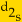
\includegraphics[width=0.6cm]{dxf2shp_converter}
 & Преобразователь DXF2Shape \index{модули!DXF2Shape}& Преобразователь файлов из формата DXF в формат SHP & Раздел \ref{dxf2shape}\\
\hline

\includegraphics[width=0.6cm]{plugin}
 & eVis & Инструмент визуализации события & Раздел \ref{sec:evis}\\
\hline

\includegraphics[width=0.6cm, height=0.6cm]{ftoolslogo}
 & fTools \index{модули!fTools}& Набор инструментов для анализа, в том числе геометрического, обработке гео-данных и исследований & Раздел \ref{sec:ftools}\\
\hline

\includegraphics[width=0.6cm]{gps_importer}
 & Инструмент GPS \index{модули!GPS}& Инструмент для загрузки и импорта данных GPS & Раздел \ref{label_plugingps}\\
\hline

\includegraphics[width=0.6cm]{grass}
 & GRASS \index{модули!инструменты GRASS} & Активация панели инструментов GRASS & Раздел \ref{sec:grass}\\
\hline

\includegraphics[width=0.6cm, height=0.6cm]{raster-info}
 & Инструменты GDAL \index{модули!GdalTools} & Растровые инструменты: упрощенный графический интерфейс для обычно используемых программ & Раздел \ref{label_plugingdaltools}\\
\hline

\includegraphics[width=0.6cm]{georeferencer}
 & Гео-привязка растров GDAL \index{модули!привязка} & Гео-привязка растровых данных с использованием GDAL & Раздел \ref{sec:georef}\\
\hline

\includegraphics[width=0.6cm]{interpolation}
 & Модуль интерполяции \index{модули!интерполяция}& Интерполяция по вершинам в векторном слое & Раздел \ref{sec:interpol}\\
\hline

\includegraphics[width=0.6cm]{mapserver_export}
 & Модуль экспорта MapServer \index{модули!экспорт в MapServer}& Экспорт файла данных проекта QGIS в формат данных MapServer & Раздел \ref{sec:mapserver_export}\\
\hline

\includegraphics[width=0.6cm]{north_arrow}
 & Указатель «Север-Юг» \index{модули!стрелка севера}& Вывод на карте указателя <<Север-Юг>> & Раздел \ref{northarrow}\\
\hline

\includegraphics[width=0.6cm]{offline_editing_copy}
 & Оффлайновое редактирование & Оффлайновое редактирование слоёв и синхронизация с базами данных & Раздел \ref{sec:offlinedit}\\
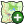
\includegraphics[width=0.6cm]{osm_load}
 & OpenStreetMap & Отображение и редактирование данных OpenStreetMap & Раздел \ref{plugins_osm}\\
\hline

\includegraphics[width=0.6cm]{oracle_raster}
 & Oracle Georaster \index{модули!georaster}& Доступ к данным  Oracle Spatial GeoRasters & Раздел \ref{sec:oracleraster}\\
\hline
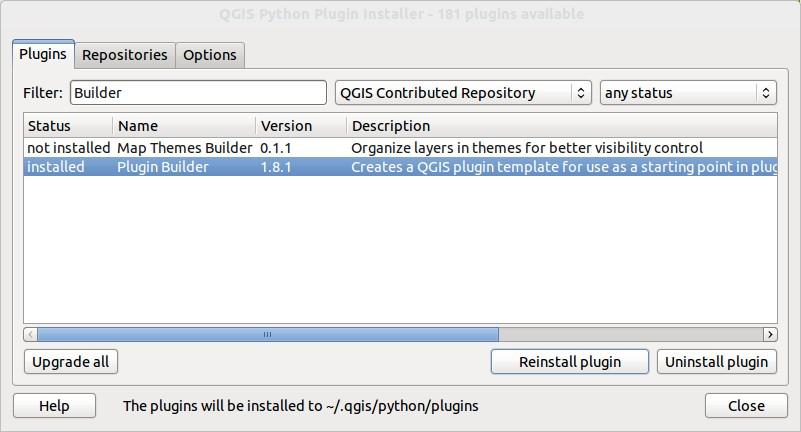
\includegraphics[width=0.6cm]{plugin_installer}
 & Установка модулей \index{модули!Plugin Installer} & Загрузка и установка модулей QGIS на языке Python & Раздел \ref{sec:python_plugin_installer}\\
\hline

\includegraphics[width=0.6cm]{raster_terrain}
 & Морфометрический анализ \index{модули!морфометрический анализ} & Расчет наклона, аспекта,
неровностей и общего искривления с использованием цифровых моделей & Раздел \ref{sec:rasterrain}\\
\hline

\includegraphics[width=0.6cm]{plugin}
 & Road graph \index{plugins!road graph} & Поиск кратчайшего маршрута на графе дорог & Раздел \ref{sec:roadgraph}\\
\hline

\includegraphics[width=0.6cm]{spiticon}
 & SPIT \index{модули!SPIT} & Инструмент импорта shp-файлов в  PostgreSQL/PostGIS & Раздел \ref{sec:loading_postgis_data}\\
\hline

\includegraphics[width=0.6cm]{plugin}
 & SQL Anywhere \index{plugins!SQL anywhere} & Работа с векторными данными в БД SQL Anywhere & Раздел \ref{sec:sqlanywhere}\\
 \hline

\includegraphics[width=0.6cm]{scale_bar}
 & Масштабная линейка \index{модули!масштабная линейка}& Отображает на карте масштабную линейку & Раздел \ref{scalebar}\\
\hline

\includegraphics[width=0.6cm]{spatialquery}
 & Пространственные запросы & Модуль пространственных запросов для векторных слоёв & Раздел \ref{sec:spatial_query}\\
\hline

\includegraphics[width=0.6cm]{mIconAddWfsLayer}
 & Модуль WFS & Добавляет возможность загрузки слоёв WFS & Раздел \ref{sec:ogc-wfs}\\
\hline
\end{longtable}}

\newpage
